This chapter introduces related work that was used in the development of this project. This chapter includes: Grounding Language Models \cref{sec:grounding_language_models}. Vision Language Models \cref{sec:vision_language_models}. Spatial Reasoning Datasets \cref{sec:spatial_reasoning_datasets}. Multimodal Transformers in \cref{sec:multimodal_transformers}. Diffusion Models in \cref{sec:diffusion_models}.

\section{Grounding Language Models} \label{sec:grounding_language_models}

Neural Language Models (LM) have shown \textbf{impressive capabilities} on many Natural Language Processing (NLP) tasks \cite{wang2019superglue, brown2020language, chowdhery2022palm}. LMs are pretrained on large corpora in order for them to learn universal language representations, which are beneficial for downstream NLP tasks and can avoid training a new model from scratch. The pretrained models are then fine-tuned in specific downstream tasks, using annotated data that is orders of magnitude smaller than the text used in the pretraining phase. Following this transfer learning methodology, researchers have extended the state of the art on a wide array of tasks as measured by leaderboards on specific benchmarks for English \cite{bommasani2021opportunities, wang2019superglue}.

Despite the impressive results of LMs for different language-related tasks, many authors criticize them for their \textbf{lack of meaning} \cite{bender2020climbing, bender2021dangers}. In their opinion, language models trained exclusively on linguistic form (i.e. words) are unable to learn meaning. Those authors suggest that \textbf{grounding is one of the key elements to bring human-like language understanding}. However, language grounding is a very broad area that covers a great diversity of techniques, modalities and concepts. In this project, we will focus on spatial reasoning, that is, \textbf{grounding LMs with spatial concepts}. We choose spatial reasoning because it is one of the most fundamental capabilities for both humans and LMs. Such relations are crucial to how humans organize the mental space and make sense of the physical world, and therefore fundamental for a grounded theory of semantics \cite{levinson2003space}. However, spatial reasoning has been found to be particularly challenging (much more challenging than capturing properties of individual entities) for current models \cite{akula2020words}.

\section{Vision Language Models} \label{sec:vision_language_models}

Vision Language Models (VLM), which are trained jointly on text and image, have been proposed as a general solution to the lack of grounding in language models \cite{lu2019vilbert, tan2020lxmert, ramesh2022hierarchical, saharia2022photorealistic}. Vision-language pre-training aims to improve performance of downstream vision and language tasks by pretraining the model on many image-text pairs. These pre-trained models can then be fine-tuned on each downstream task.

VLMs have been used in tasks that require grounding spatial concepts, such as VQA \cite{antol2015vqa} or NLVR2 \cite{suhr2018corpus}, but recent work has shown that \textbf{VLMs struggle to ground spatial concepts properly} \cite{liu2022things}. Large generative VLMs trained on massive amounts of data like DALLE-2 \cite{ramesh2022hierarchical} or IMAGEN \cite{saharia2022photorealistic} are known to possess visual-reasoning skills \cite{cho2022dall}, but they are not publicly available and only accessible to large companies.

There are several \textbf{works that try to ground language models to spatial relations}. For example, \cite{bagherinezhad2016elephants, elazar2019large} focus on the acquired commonsense knowledge of models about object scales, e.g. do they know that a person is bigger than an ant? However, they ask about generic object scale relations, without providing any context. Some other authors \cite{collell2018acquiring, elu2021inferring} work on implicit and explicit spatial relations of objects, given some descriptive texts. The proposed benchmark datasets are designed for object bounding box generation.

\section{Synthetic Visual Reasoning Datasets} \label{sec:synthetic_visual_reasoning_datasets}

% add example images?   

Multimodal training datasets with images and descriptions that include spatial relations tend to be small. Synthetic visual reasoning datasets have been proposed to overcome this problem. These datasets enable full control of dataset generation, easing spatial reasoning capability probing  on VLMs. Some examples of synthetic datasets include SHAPES \cite{andreas2016neural}, CLEVR \cite{liu2019clevr}, NLVR \cite{suhr-etal-2017-corpus} and SPARTQA \cite{mirzaee-etal-2021-spartqa}.

\textbf{SHAPES} is a dataset of synthetic images designed to benchmark understanding of spatial and logical relations among multiple objects \cite{andreas2016neural}. The dataset consists of complex yes or no questions about arrangements of colored shapes. Each image is a 3×3 grid of objects. Each object is characterized by shape (circle, square, triangle), colour (red, green, blue) and size (small, big).

\textbf{CLEVR} was one of the pioneering works on testing \textbf{compositional language and elementary visual reasoning} \cite{johnson2017clevr}. However, it presents two major drawbacks: i) questions not only cover spatial grounding but some other concepts such as compositional language and attribute identification, and ii) spatial relations are limited to four, i.e. left, right, behind and in front. 

\textbf{NLVR} containins natural language sentences grounded in images \cite{suhr-etal-2017-corpus}. The task is to determine whether a sentence is true about a visual input. The data was collected through crowdsourcing, and solving the task requires reasoning about sets of objects, comparisons, and spatial relations.

\textbf{SPARTQA} provides a synthetic \textbf{question-answering} dataset that is specially focused on spatial reasoning capabilities \cite{mirzaee-etal-2021-spartqa}. SPARTQA is built on NLVR’s images containing more objects with richer spatial structures. However, it contains only text and no images, and therefore it does not provide any means to ground spatial concepts.

A very recent work proposes a method called \textbf{Pseudo-Q} to \textbf{automatically create synthetic datasets} that can be used to train visually grounded models \cite{jiang2022pseudo}. Their method consists of leveraging an off-the-shelf object detector to identify visual objects from unlabeled images, and then creating language queries for these objects that are obtained in an unsupervised fashion with a pseudo-query generation module.

The major drawback of synthetic datasets is that they do not always accurately reflect the challenges of reasoning in the real world. Some aspects that are very important in the real world are not taken into account in synthetic images. For example, the orientations of objects, their context and the viewpoint can affect their spatial relation.

\section{Natural Visual Reasoning Datasets}

Many vision-language datasets with natural images also contain spatial relations. For example, NLVR2 \cite{suhr2018corpus}, MS COCO \cite{lin2014microsoft}, and VQA \cite{antol2015vqa}.

\textbf{NLVR2} is a dataset for joint reasoning about natural language and images, with a focus on semantic diversity, compositionality, and visual reasoning challenges \cite{suhr2018corpus}. There are 9 prevalent linguistic challenges in NLVR2 among which are spatial relations.
The examples in \cref{fig:nlvr2_examples} require addressing challenging semantic phenomena.

\begin{figure}[ht]
  \centering
    \centering
    \begin{subfigure}[b]{0.49\linewidth}
    \centering
    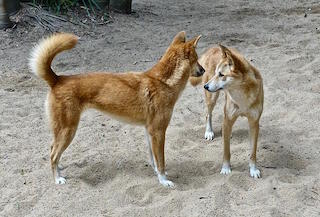
\includegraphics[width=0.49\linewidth]{images/nlvr_ex_0_img_0.jpg}
    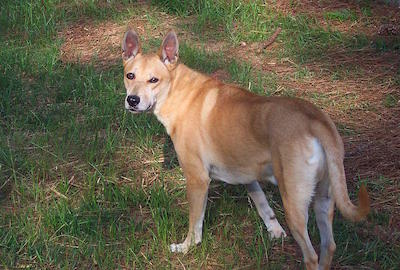
\includegraphics[width=0.49\linewidth]{images/nlvr_ex_0_img_1.jpg}
    \caption{The left image contains twice the number of dogs as the right image, and at least two dogs in total are standing.}
     \end{subfigure}
     \hfill
     \begin{subfigure}[b]{0.49\linewidth}
     \centering
    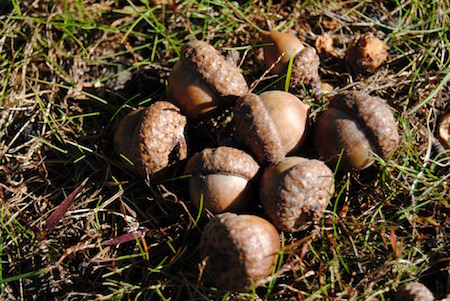
\includegraphics[width=0.49\linewidth]{images/nlvr_ex_1_img_0.jpg}
    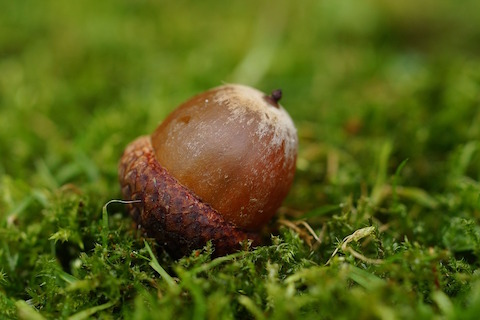
\includegraphics[width=0.49\linewidth]{images/nlvr_ex_1_img_1.jpg}
    \caption{One image shows exactly two brown acorns in back-to-back caps on green foliage.}
     \end{subfigure}
    \caption{Two examples from NLVR2, where each caption is paired with two images. The first caption is True and the second one is False.}
    \label{fig:nlvr2_examples}
\end{figure}

\textbf{VQA} \cite{antol2015vqa} is a popular vision and language task. Given an image and a question about the image, the task is to provide an accurate answer. VQA is commonly used as a benchmark to evaluate VQA systems. Questions are generally open-ended but multiple choices are provided for some questions. Some examples are shown in \cref{fig:vqa_examples}.

\begin{figure}[ht]
    \centering
    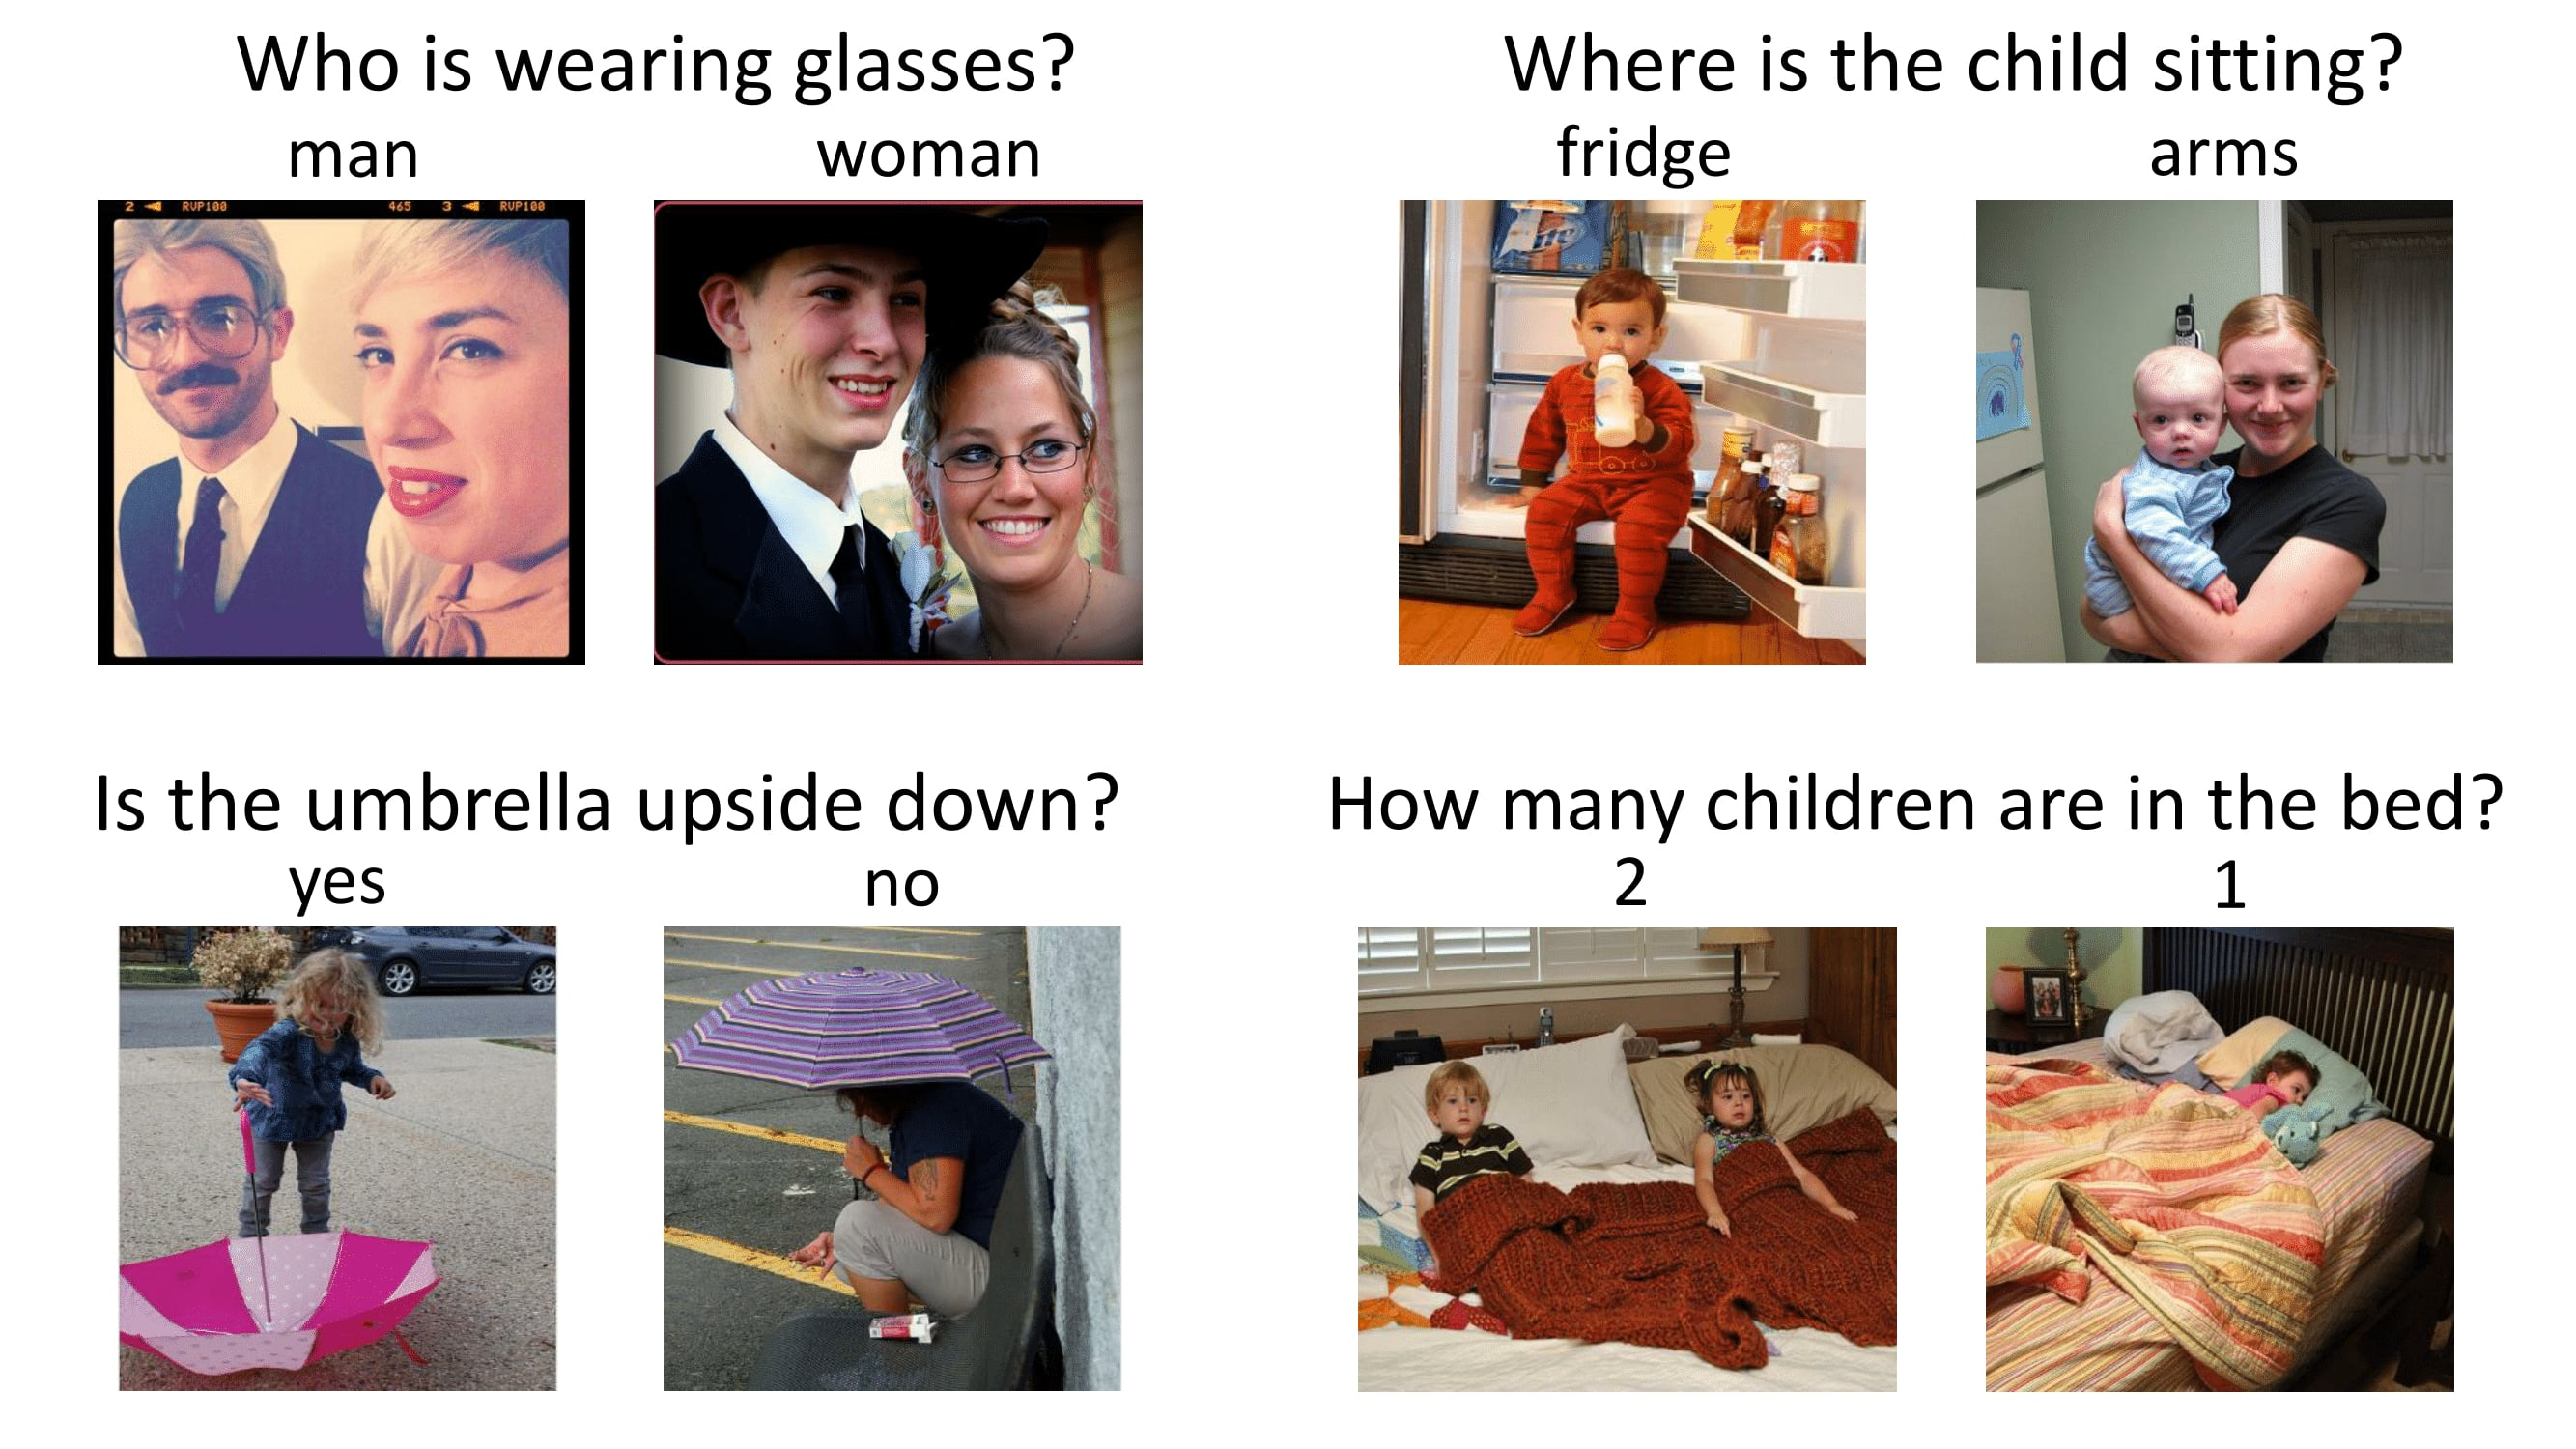
\includegraphics[width=\linewidth]{images/vqa_examples.jpg}
    \caption{Example images, questions and answers from VQA.}
    \label{fig:vqa_examples}
\end{figure}

The problem of these datasets is that many different challenges are mixed. Sentences have complex lexical and syntactic information. This makes it hard to identify the exact challenges, preventing categorised analysis.

With the objective of \textbf{evaluating spatial relations}, a recent work provides new unified datasets \cite{liu2022things}. As the objective of such work is to evaluate whether VLMs learn more spatial commonsense than LMs, the datasets are purely textual, so they do not provide any means to ground spatial concepts. Interestingly, authors find that VLMs, and more concretely text-to-image systems, perform much better than text-only LMs.

\section{Visual Spatial Reasoning Datasets} \label{sec:spatial_reasoning_datasets}

The \textbf{Winoground} dataset \cite{thrush2022winoground} is focused on \textbf{evaluating visio-linguistic compositional reasoning} in VLMs. Each instance in the dataset is composed of two images and two captions, but crucially, both captions contain a completely identical set of words, only in a different order. The task is then to match them correctly, which requires the systems to properly deal with composition in natural language. Previous works have shown that language transformers have \textbf{difficulties in learning word order} \cite{sinha2020unnatural,sinha2021matterslittle}. Winoground provides a means to test whether this is also true for multimodal models.

Another very recent dataset named \textbf{Visual Spatial Reasoning (VSR)} \cite{liu2022visual}, whose objective is to test spatial grounding capabilities by covering 65 different spatial relations over natural images collected from COCO \cite{lin2014microsoft}. Given an image, VSR provides a caption which describes a spatial relation between two of the objects that appear in the image. That relation can be real or fake, and that is precisely what the model has to infer, i.e. whether the caption is correct with respect to the given image. Another advantage of this dataset is that it is annotated by humans. Given its features, \textbf{we believe VSR is a good candidate to evaluate spatial grounding in LMs}.

\section{Multimodal Transformers} \label{sec:multimodal_transformers}

Multimodal transformers are state-of-the-art in many vision-language tasks, and that includes spatial reasoning. Most of the models tested in Winoground \cite{thrush2022winoground} and VSR \cite{liu2022visual} are multimodal transformers. Those transformers differ in embedding, architecture and pretraining objectives and cross-modal attention.

\paragraph{Embedding.} Most models use a pretrained BERT tokenizer for text encoding. For image embedding, there are more different options. Some models use Convolutional Neural Networks (CNN) to extract features from images. Another common approach is to use Vision Transformer (ViT).

\paragraph{Architecture.} Depending on their architecture, they can mainly be classified into two types: single-stream and dual-stream transformers. On the one hand, in \textbf{single-stream} transformers the image and text embeddings are concatenated and then jointly encoded. On the other hand, \textbf{dual-stream} transformers have two separate modality-specific encoders with optional cross-modality fusion.

\paragraph{Pretraining Objectives.} Vision-language transformers use a different pretraining objectives including \textbf{masked language modeling} (MLM), image-conditioned \textbf{language modeling} (LM), \textbf{image-text contrastive} learning (ITC), \textbf{image-text matching} (ITM). For example, BLIP \cite{li2022blip} is jointly pre-trained with three vision-language objectives: ITC, ITM and LM.

\paragraph{Cross-Modal Attention.} There are different types of multimodal attention as presented in \cite{hendricks2021decoupling}. In \textbf{modality-specific attention}, the language and visual input attend to their modality. In \textbf{merged attention}, the language and visual input attend to both themselves and the other modality. In \textbf{co-attention}, the language and visual input only attends to the other modality input.

\section{Diffusion Models} \label{sec:diffusion_models}

Diffusion models are machine learning systems trained to denoise random gaussian noise step by step, to get to a sample image. Neural networks are trained to predict a way to slightly denoise the picture in each step. As we can see in \cref{fig:diffusion_process}, after a certain number of steps, a sample is obtained.

\begin{figure}[ht]
    \centering
    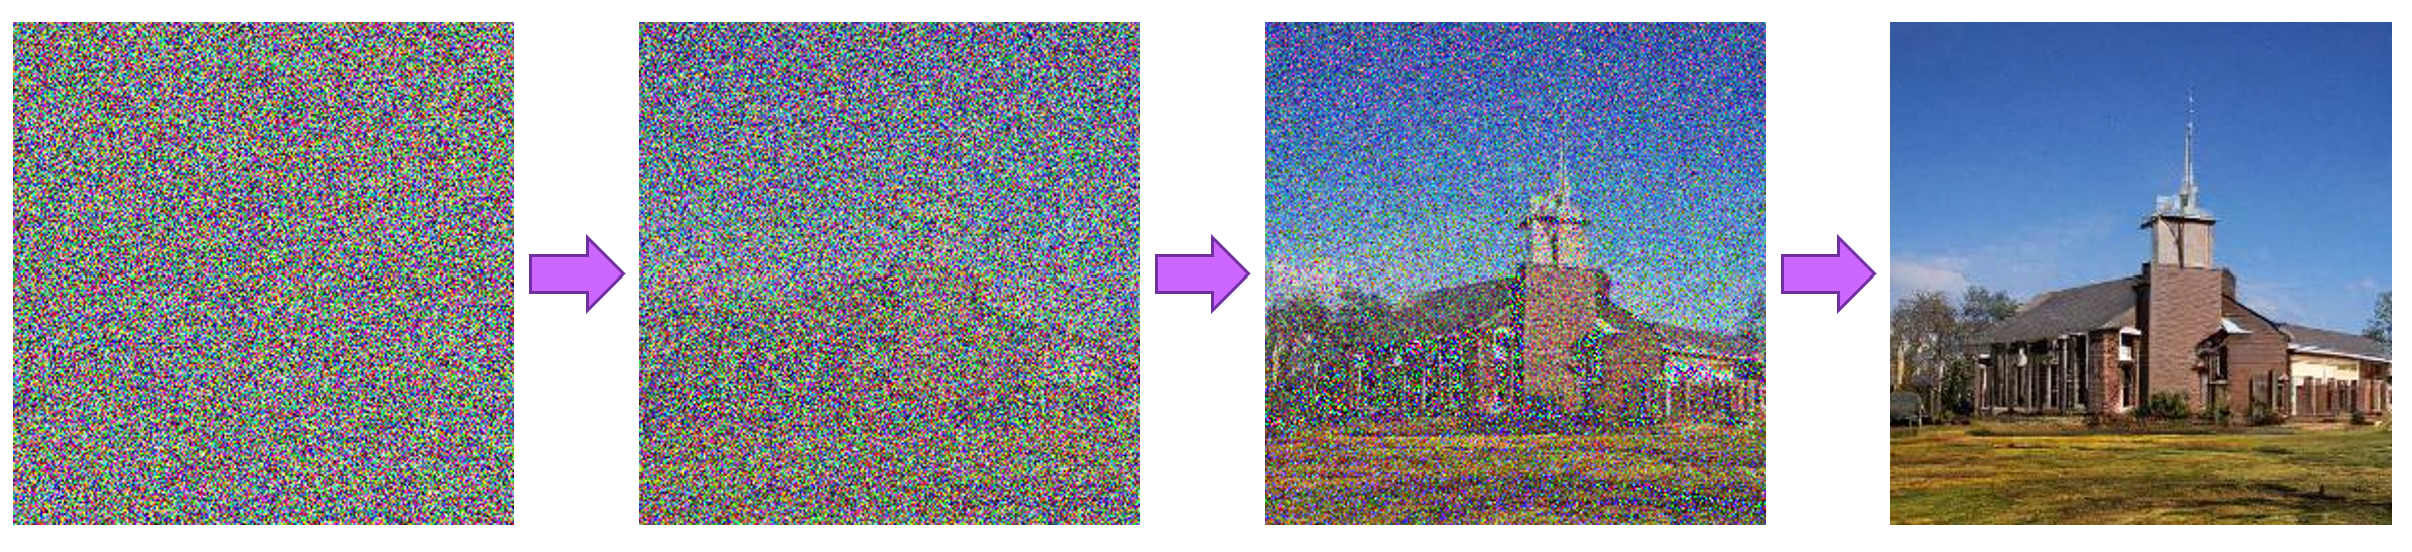
\includegraphics[width=\linewidth]{images/diffusion-process.png}
    \caption{In the diffusion process random images are denoised in multiple steps to get a sample image. Source: \url{https://github.com/huggingface/notebooks/blob/main/diffusers/diffusers_intro.ipynb}}
    \label{fig:diffusion_process}
\end{figure}

Diffusion models have obtained SOTA results on image generation. However, one downside of diffusion models is that the reverse denoising process is slow. In addition, these models consume a lot of memory because they work in pixel space. Therefore, it is challenging to train these models and also to use them for inference.

Consequently, most of the recent diffusion models, e.g. DALLE-2 \cite{ramesh2022hierarchical} and IMAGEN \cite{saharia2022photorealistic}, are unfortunately not accessible to the community. The most popular exception is Stable Diffusion \cite{rombach2021highresolution}, which has been open sourced and can be used on a single GPU.

\subsection{Stable Diffusion}

Stable Diffusion is based on a type of diffusion model called Latent Diffusion \cite{rombach2021highresolution}. Latent diffusion reduces the memory and compute complexity by applying the diffusion process over a lower dimensional latent space. There are three main components in latent diffusion: an autoencoder (VAE), a U-Net and a text-encoder (CLIP).

\paragraph{The autoencoder (VAE) \cite{kingma2013auto}.} The VAE has two parts, an encoder and a decoder, as we can see in \cref{fig:vae}. During latent diffusion training, the encoder maps the images to a latent space for the forward diffusion process, which applies more noise at each step. During inference, the decoder maps the latents generated by the reverse diffusion process back to the images. The encoder and decoder are trained jointly to minimize the reconstruction error.

\begin{figure}[ht]
    \centering
    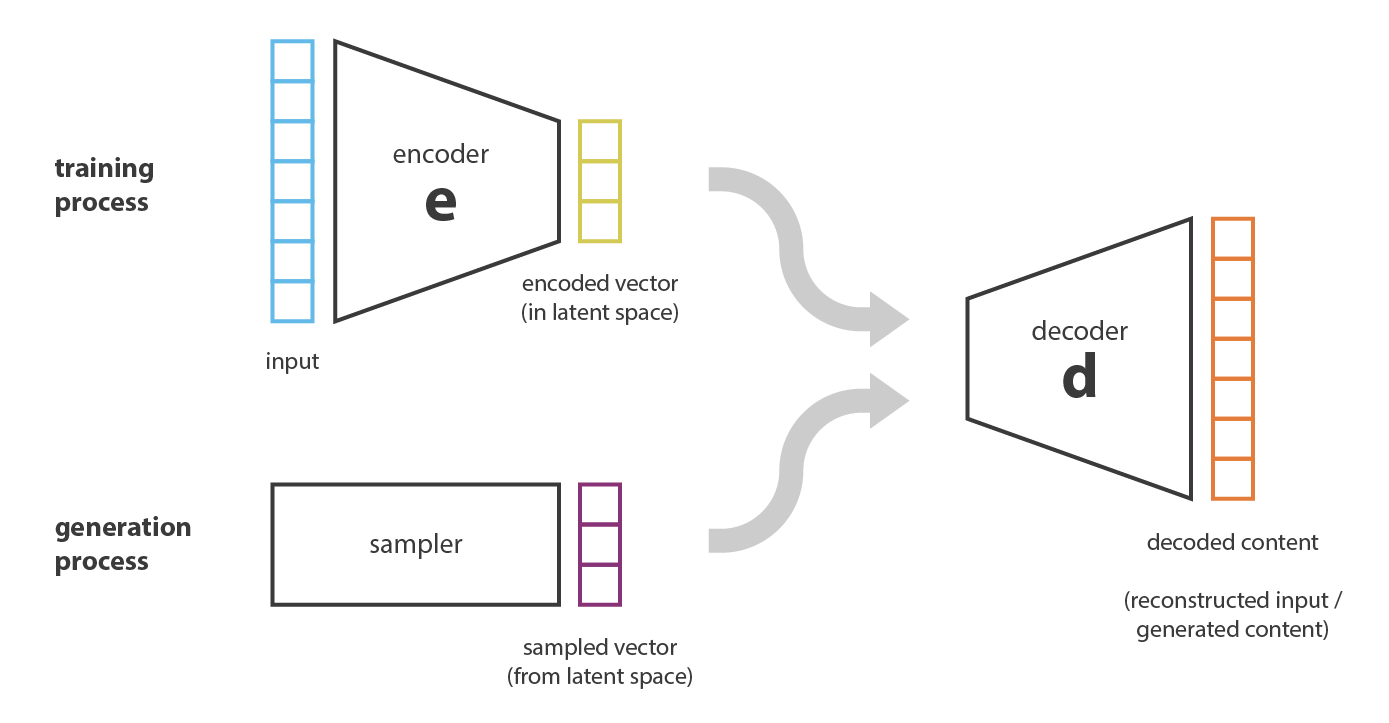
\includegraphics[width=\linewidth]{images/vae.png}
    \caption{Variational Autoencoder (VAE) training and generation processes. Source: \url{https://towardsdatascience.com/understanding-variational-autoencoders-vaes-f70510919f73}}
    \label{fig:vae}
\end{figure}

\paragraph{The U-Net \cite{ronneberger2015u}.} The U-Net also has an encoder part and a decoder part, as shown in \cref{fig:unet_model}. The encoder has several ResNet blocks which half the image size by 2. The decoder does the opposite process to upsample the image to the initial size. The U-Net outputs the noise residual which can be used to compute the denoised image representation. To prevent the U-Net from losing important information while downsampling, shortcut connections are usually added from the downsample path to the corresponding layers in the upsample path. Moreover, the output of the stable diffusion U-Net is conditioned on text-embeddings via cross-attention layers.

\begin{figure}[ht]
    \centering
    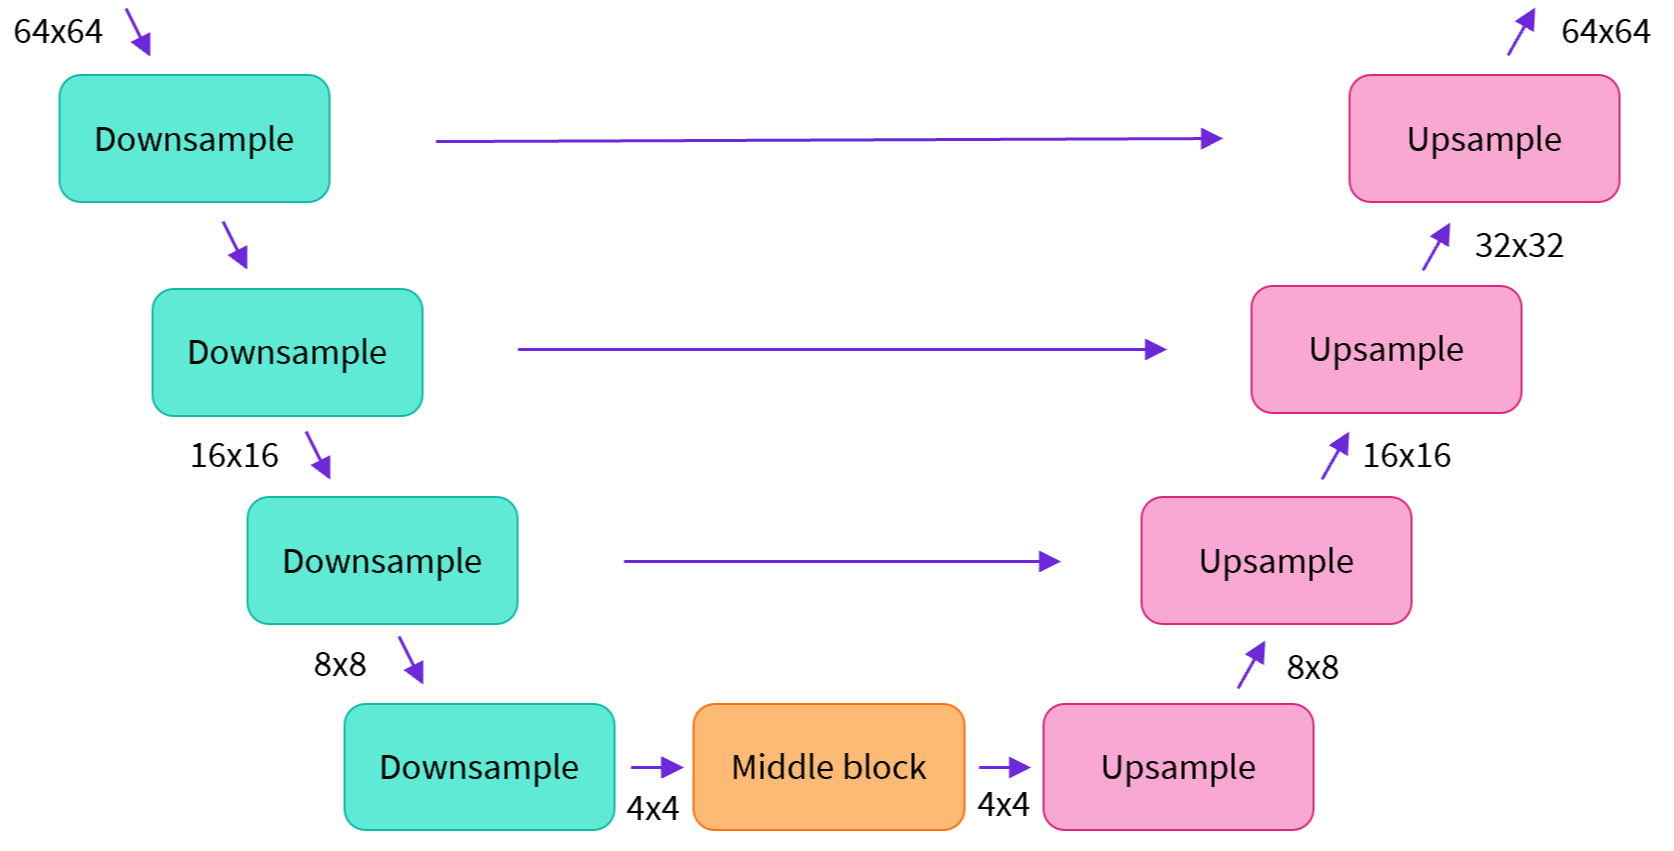
\includegraphics[width=\linewidth]{images/unet-model.png}
    \caption{The architecture of the U-Net model. Source: \url{https://github.com/huggingface/notebooks/blob/main/diffusers/diffusers_intro.ipynb}}
    \label{fig:unet_model}
\end{figure}

\paragraph{The text-encoder (CLIP) \cite{radford2021clip}.} The text-encoder transforms the input prompt into an embedding for the U-Net. Stable Diffusion does not train the text-encoder during training and uses an already trained CLIP text encoder, which is shown in \cref{fig:clip}.

\begin{figure}[ht]
    \centering
    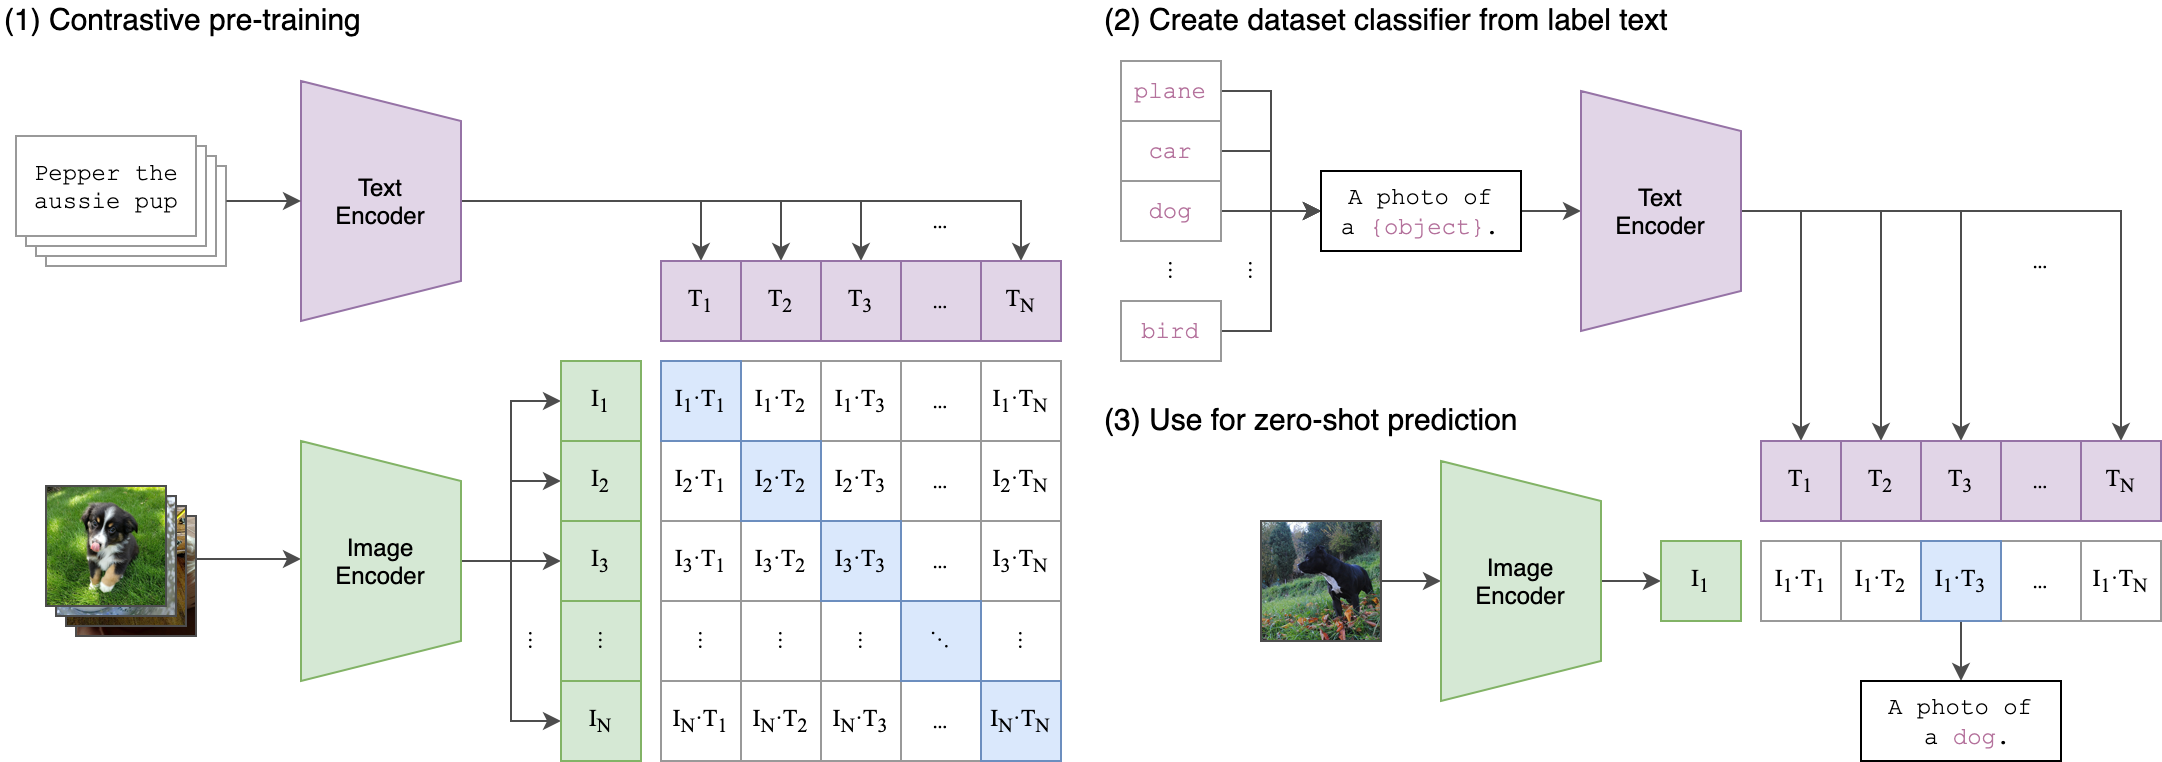
\includegraphics[width=\linewidth]{images/clip.png}
    \caption{CLIP model architecture. Source: \url{https://github.com/openai/CLIP}}
    \label{fig:clip}
\end{figure}

With the previous components we nearly have the full Stable Diffusion inference architecture \cref{fig:stable_diffusion}. The stable diffusion model takes a latent seed and a text prompt as input. The latent seed is  used to generate initial random latents. The output of the U-Net is used to compute a denoised image representation with a scheduler algorithm. This process is repeated many to get better representations in each iteration. Finally, the latent image representation is decoded by the VAE decoder.

\begin{figure}[ht]
    \centering
    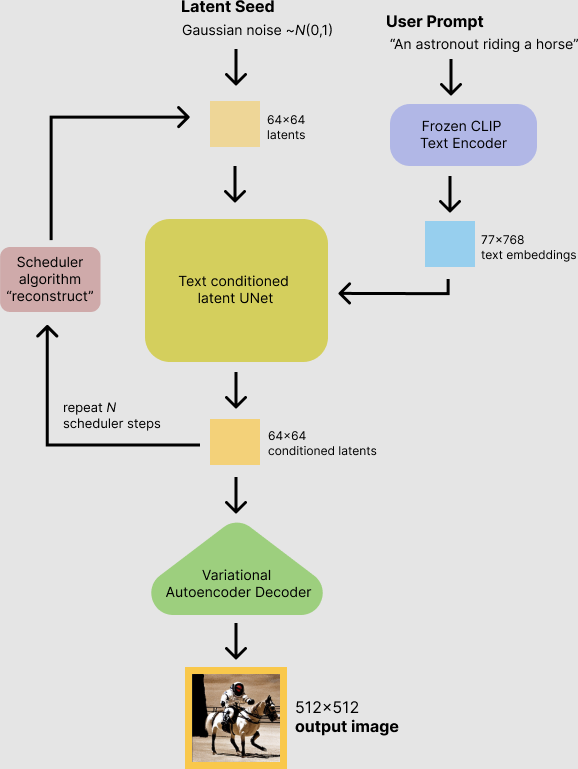
\includegraphics[width=0.6\linewidth]{images/stable_diffusion.png}
    \caption{Stable Diffusion inference architecture. Source: \url{https://github.com/huggingface/notebooks/blob/main/diffusers/stable_diffusion.ipynb}}
    \label{fig:stable_diffusion}
\end{figure}